\documentclass{lab}

\renewcommand{\AA}{\ensuremath{\mathring{A}}}

\begin{document}

\labtitle{5.4.2}{Исследование энергетического спектра $\beta$-частиц и определение их максимальной энергии при помощи магнитного спектрометра}{3~октября~2019~г.}{10~октября~2019~г.}

\section*{Постановка эксперимента}

\begin{quote}
	\textbf{{\normalsize Цель работы: }}
	С помощью магнитного спектрометра исследовать энергетический спектр $ \beta $-частиц при распаде ядер $ ^{137} $Cs и определить их максимальную энергию.
\end{quote}

\begin{quote}
	\textbf{{\normalsize Оборудование: }}
	$ \beta $-спектрометр с короткой магнитной линзой.
\end{quote}

\section*{Теория}
	Бета-распадом называется самопроизвольное превращение ядер, при котором их массовое число не изменяется, а заряд увеличивается или уменьшается на единицу. Бета-активные ядра встречаются во всей области значений массового числа $A$, начиная от единицы (свободный нейтрон) и кончая самыми тяжелыми ядрами. Период полураспада $\beta$-активных ядер изменяется от ничтожных долей секунды до $10^{18}$ лет. Выделяющаяся при единичном акте $\beta$-распада энергия варьируется от 18 кэВ (для распада трития ${}_1^3H$) до 13,4 МэВ (для распада изотопа бора ${}_5^{12}B$).
	В данной работе мы будем иметь дело с электронным распадом 
	\begin{equation*}
	{}_Z^AX \longrightarrow {}_{Z+1}^AX + e^{-} + \tilde \nu,
	\end{equation*}
	при котором кроме электрона испускается антинейтрино. Освобождающаяся при $\beta$-распаде энергия делится между электроном, антинейтрино и дочерним ядром, однако доля энергии, передаваемой ядру, исчезающе мала по сравнению с энергией, уносимой электроном и антинейтрино. Практически можно сказать, что эти две частицы делят между собой всю освобождающуюся энергию. Поэтому электроны могут иметь любое значение энергии -- от нулевой до некоторой максимальной, которая равна энергии, освобождающейся при $\beta$-распаде, и является важной физической величиной. 
	
	Вероятность $dw$ того, что при распаде электрон вылетит с импульсом $d^3 \vec{p}$, а антинейтрино с импульсом в интервале $d^3 \vec{k}$, очевидно, пропорциональна произведению этих дифференциалов. Нужно также учесть закон сохранения энергии, согласно которому импульсы $\vec{p}$ и $\vec{k}$ электрона и антинейтрино связаны соотношением 
	\begin{equation} \label{E_save}
	E_e - E - ck = 0,
	\end{equation}
	где $E_e$ -- максимальная энергия электрона, кинетическая энергия электрона $E$ связана с его импульсом обычным релятивистским соотношением 
	\begin{equation}
	E = c \sqrt{p^2 + m^2 c^2} - m c^2, 
	\end{equation}
	а через $ck$ обозначена энергия антинейтрино с импульсом $k$. Условие (\ref{E_save}) можно учесть введением в выражение для $dw$ $\delta$-функции
	\begin{equation}
	\delta (E_e - E - ck), 
	\end{equation}
	по определению не равной нулю только при соблюдении условия (\ref{E_save}).
	
	Таким образом, вероятность $dw$ может быть записана в виде
	\begin{equation}
	dw = D \delta (E_e - E - ck) \  d^3 \vec{p} \  d^3 \vec{k} =  D \delta (E_e - E - ck) \ p^2 dp \ k^2 dk \ d\Omega_e \ d\Omega_{\tilde \nu}, 
	\end{equation}
	где $D$ -- некоторый коэффициент пропорциональности, $d\Omega_e,\ d\Omega_{\tilde \nu}$ -- элементы телесных углов направлений вылета электрона и нейтрино. Вероятность $dw$ непосредственно связана с $\beta$-спектром, поскольку для очень большого числа $N_0$ распадов число $dN$ распадов с вылетом электроноа и антинейтрино с импульсами соответственно от $\vec{p}$ до $\vec{p} + d\vec{p}$ и от $\vec{k}$ до $\vec{k} + d\vec{k}$ определяется соотношением 
	\begin{equation}
	dN = N_0 dw.
	\end{equation}
	Коэффициент $D$ в формуле (\ref{E_save}) с хорошей точностью можно считать для рассматриваемых нами распадов константой.
	
	Величину $dw$ можно проинтегрировать по всем углам и по абсолютному значению импульса нейтрино. Интегрирование по каждому телесному углу дает множитель $4 \pi$, а 
	\begin{equation}
	\int_{- \infty} ^{+ \infty} f(x) \delta (x) dx = f(0).
	\end{equation}
	Поэтому, после домножения $dw$ на $N_0$ имеем
	\begin{equation} \label{p-dist}
	dN = \frac{16 \pi^2 N_0}{c^2}Dp^2(E_e - E)^2 dp, 
	\end{equation}
	где $dN$ обозначает уже число электронов, вылетающих из ядра с импульсом, величина которого лежит между $p$  и $p + dp$.
	
	Чтобы получить распределение электронов по энергиям, надо в (\ref{p-dist}) перейти от $dp$ к $dE$:
	\begin{equation}
	dE = \frac{c^2 p}{E + mc^2} dp,
	\end{equation}
	после чего выражающая форму $\beta$ спектра величина $N(E) = dN/dE$ приобретает вид
	\begin{equation} \label{E-dist}
	\frac{dN}{dE} = N_0 B c p (E + mc^2)(E_e - E)^2 = N_0 B \sqrt{E (E + 2mc^2)} (E_e - E)^2 (E + mc^2), 
	\end{equation}
	где $B = (16 \pi^2 / c^4) D$. В нерелятивистском приближении, которое и имеет место в нашем случае, выражение (\ref{E-dist}) упрощается, и мы имеем
	\begin{equation} \label{non-rel-E-dist}
	\frac{dN}{dE} \approx \sqrt{E} (E_e - E)^2.
	\end{equation}
	
	\begin{wrapfigure}{r}{0.5\linewidth}
		\vspace{-5ex}  
		\center{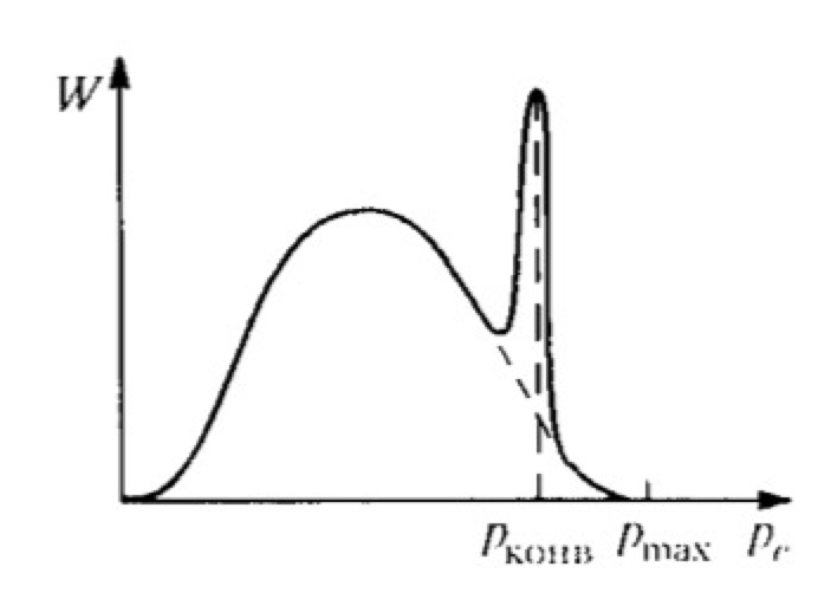
\includegraphics[width=.7\linewidth]{dist.png}}
		\caption{Форма спектра $\beta$-частиц}
		\label{dist-pic}
	\end{wrapfigure}
	
	Дочерние ядра, возникающие в результате $\beta$-распада, нередко оказываются возбужденными. Возбужденные ядра отдают свою энергию либо излучая $\gamma$-квант, либо передавая избыток энергии одному из электронов с внутренних оболочек атома. Излучаемые в таком процессе электроны имеют строго определенную энергию и называются конверсионными.
	
	Итоговая форма спектра представлена на рис. \ref{dist-pic}. 
	Спектр имеет вид широкого колокола с резким конверсионным максимумом, ширина которого определяется исключительно разрешающей способностью прибора. Кривая плавно отходит от нуля и столь же плавно, по параболе, касается оси абсцисс в области максимальной энергии электронов $E_e$. 
	
\section*{Экспериментальная установка}

	\begin{figure}[ht!]
		\center{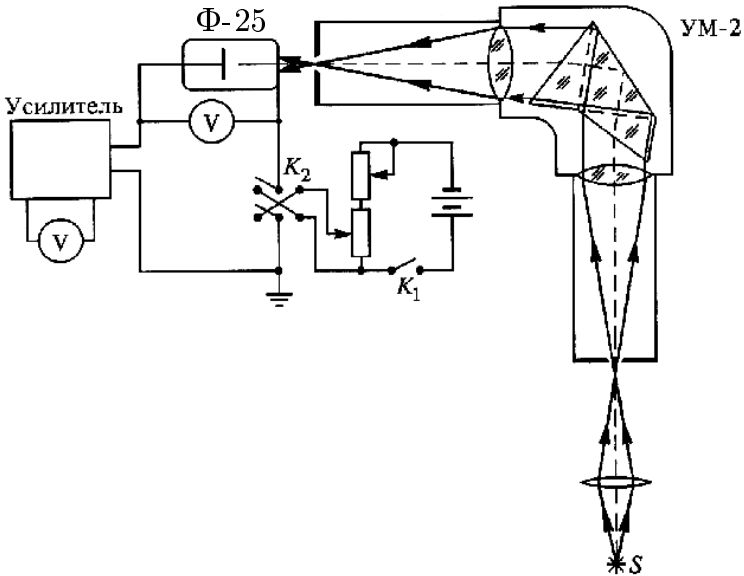
\includegraphics[width=\linewidth]{scheme.png}}
		\caption{Схема установки}
		\label{scheme}
	\end{figure}
	
	Энергию $\beta$-частиц определяют с помощью $\beta$-спектрометров. В работе используются магнитный спектрометр с "короткой линзой". Его схема представлена на рис. \ref{scheme}. Электроны, испускаемые радиоактивным источником, попадают в магнитное поле катушки, ось которой параллельна оси $OZ$ (оси симметрии прибора). Траектории электронов в магнитном поле представляют собой сложные спирали, сходящиеся за катушкой в фокусе, расположенном на оси $OZ$. В фокусе установлен детектор электронов.
	
	Как показывает расчет, для заряженных частиц тонкая катушка эквивалентна линзе. Ее фокусное расстояние $f$ зависит от импульса электронов $p_e$ и от индукции магнитного поля линзы (т.е. от силы тока $I$, протекающего через катушку) следующим образом:
	\begin{equation} \label{focus}
	\frac{1}{f} \propto \frac{I^2}{p_e^2}
	\end{equation}
	
	При заданной силе тока на входное окно счетчика фокусируются электроны с определенным импульсом. Электроны, обладающие другими значениями импульса, при этом не сфокусированы и в основном проходят мимо окна. При изменении тока в катушке на счетчик последовательно фокусируются электроны с разными импульсами. Так как геометрия прибора в течение опыта остается неизменной, импульс сфокусированных электронов пропорционален величине тока $I$:
	\begin{equation}
	p_e = kI.
	\end{equation}
	
	Рассмотрим связь между числом частиц, регистрируемых установкой, и функцией $W(p_e) = dW_e/dp_e$, определяемой формулой (\ref{non-rel-E-dist}). Как легко понять, 
	\begin{equation}
	N(p_e) \simeq W(p_e) \Delta p_e,
	\end{equation}
	где $\Delta p_e$~---~разрешающая способность спектрометра. Формула (\ref{focus}) показывает, что при заданном токе фокусное расстояние магнитной линзы зависит от импульса частиц. Мимо счетчика проходят частицы, для которых фокусное расстояние линзы слишком сильно отличается от нужного, т.е. при недопустимо больших $\Delta f$. Дифференцируя формулу (\ref{focus}) при постоянном токе, найдем:
	\begin{equation}
	\Delta p_e = \frac{1}{2} \frac{\Delta f}{f} p_e.
	\end{equation}
	Таким образом, величина интервала $\Delta p_e$, регистрируемого спектрометром, пропорциональна величине импульса. Окончательно получаем:
	\begin{equation}
	N(p_e) = C W(p_e) p_e, 
	\end{equation}
	где $C$~---~некоторая константа.



\section*{Выполнение работы}

Снимем зависимость $ N(p) $: распределение электронов по импульсу. Затем рассмотрим эту зависимость при линеаризации нужной области, используем график Ферми для получения $ E_e $ -- максимальной энергии $ \beta $-частиц при распаде $ ^{137} $Cs.

\begin{figure}[H]
	\centering
	\begin{tikzpicture}
	
	\pgfplotstableread{
		X		Y		x-err	y-err
		81		0.01		00		0
		142		-0.19		00		0
		198		0.09		00		0
		275		0.95		00		0
		338		1.05		00		0
		393		2.13		00		0
		412		3.04		00		0
		457		3.75		00		0
		519		3.81		00		0
		552		4.83		00		0
		591		5.12		00		0
		612		5.23		00		0
		652		5.17		00		0
		693		4.97		00		0
		709		4.43		00		0
		783		3.87		00		0
		803		2.86		00		0
		844		2.01		00		0
		891		1.83		00		0
		908		1.83		00		0
		943		3.00		00		0
		991		4.01		00		0
		1000	6.23		00		0
		1012	8.34		00		0
		1039	7.48		00		0
		1093	5.06		00		0
		1105	2.87		00		0
		1192	0.12		00		0
		1226	-0.89		00		0
	}{\mytable}
	
	\begin{axis}[
	width = 0.8\textwidth,
	grid = major,
	xlabel = $ p_e \text{, кэВ/с} $,
	ylabel = $ N - N_{\text{фон}} $,
	xmin = 0,
	xmax = 1400,
	ymin = -2,
	ymax = 10
	]
	
	\addplot[
	only marks,
	color = red,
	mark = *,
	error bars/.cd,
	x dir = both,
	x explicit,
	y dir = both,
	y explicit
	]
	table[
	x error = x-err,
	y error = y-err
	] {\mytable};
	
	\end{axis}
	\end{tikzpicture}
	\caption{Распределение электронов по импульсу}
	\label{g_1}
\end{figure}

\begin{figure}[H]
	\centering
	\begin{tikzpicture}
	
	\pgfplotstableread{
		X		Y		x-err	y-err
		002		376	0	0
		044		152	0	0
		098		170	0	0
		137		197	0	0
		151		200	0	0
		172		197	0	0
		212		163	0	0
		246		161	0	0
		263		164	0	0
		297		150	0	0
		314		138	0	0
		348		124	0	0
		365		114	0	0
		423		086	0	0
		450		069	0	0
		479		053	0	0
		502		050	0	0
		547		049	0	0
		562		059	0	0
		596		067	0	0
		604		077	0	0
		619		083	0	0
		650		076	0	0
		682		056	0	0
		706		048	0	0
		764		016	0	0
		840		007	0	0
	}{\mytable}

	\pgfplotstableread{
		X		Y		x-err	y-err
		263		164	0	0
		297		150	0	0
		314		138	0	0
		348		124	0	0
		365		114	0	0
		423		086	0	0
		450		069	0	0
		479		053	0	0
	}{\table}
	
	\begin{axis}[
	width = 0.8\textwidth,
	grid = major,
	xlabel = $ T \text{, кэВ} $,
	ylabel = $ mk~Fermi $,
	xmin = 0,
	xmax = 900,
	ymin = 0,
	ymax = 400
	]
	
	\addplot[
	only marks,
	color = red,
	mark = *,
	error bars/.cd,
	x dir = both,
	x explicit,
	y dir = both,
	y explicit
	]
	table[
	x error = x-err,
	y error = y-err
	] {\mytable};
	
	\addplot[
	mark = none,
	color = red
	]
	table[
	y = {create col/linear regression={y=Y}}
	] % compute a linear regression from the
	{\table};
	
	\addplot[no marks,red,domain=-100:600]{\pgfplotstableregressiona*x+\pgfplotstableregressionb};
	
	\end{axis}
	\end{tikzpicture}
	\caption{График Ферми}
	\label{g_2}
\end{figure}

Из графика Ферми получаем $E_e = 602 \pm 3 \text{ кэВ}$.

\subsection*{Итоги}

В работе был исследован спектр $\beta$-распада ядра ${}^{137}$Cs. Полученная форма спектра совпадает с предсказанной теоретически. Из графика Ферми получено значение $E_e~=~602~\pm~3~\text{ кэВ}$, согласующееся с табличным значением $514 \text{ кэВ}$ по порядку величины. 

Возможной причиной отличия полученной величины от справочной является фоновое излучение, которое могло меняться во время эксперимента и отличаться от измеренного в конце.

Кроме того, на экспериментальной установке стоял дефектный вакуумметр, в следствие чего было невозможно определить, достиг ли вакуум в спектрометре нужного значения.

\end{document}